\documentclass[a4paper,french]{paper}
\usepackage{../../_latex_assets/villemejane_iogs_ceti}

%Informations about this document 
%------------------------------------------
\def\module{Conception Electronique pour le Traitement de l'Information}
\def\moduleAbrege{5N-027-SCI / CéTI}
\def\annee{}

\def\titre{Bloc 2 / Filtrage actif}
\author{Julien VILLEMEJANE}

\subtitle{Bloc 2}
\institution{LEnsE / Institut d'Optique Graduate School}

\title{\titre}
\begin{document} 
%Beginning First Page. 
%------------------------------------------
\enteteThematiqueObligatoire{}

%Beginning Content. 
%------------------------------------------

%%%%%%%%%%%%%%%%%%%
\encadreTDExo{1 - Filtrer une composante fréquentielle}{
Proposer une structure de filtre du premier ordre qui laisse passer des signaux au dessus d'une fréquence $f_c$. Donner les principales caractéristiques et limitations d'un tel filtre.
}


%%%%%%%%%%%%%%%%%%%
\encadreTDExo{2 - Filtrer une composante fréquentielle}{
On se propose d'étudier la structure suivante :

\begin{center}
	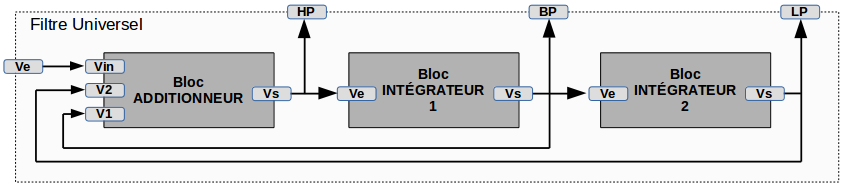
\includegraphics[width=14cm]{images/universel_structure.png}
\end{center}

Pour cela, on se propose d'étudier les deux circuits suivants :

\begin{center}
Intégrateur

	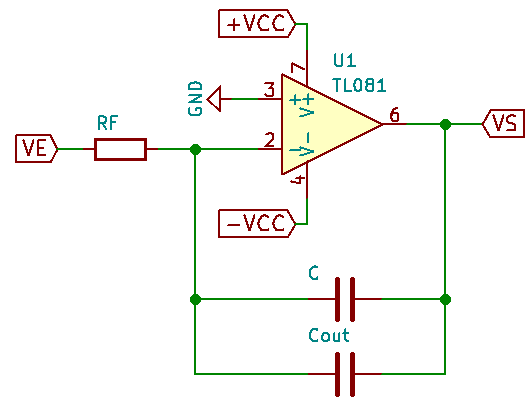
\includegraphics[width=8cm]{images/universel_integrateur.png}

Additionneur

	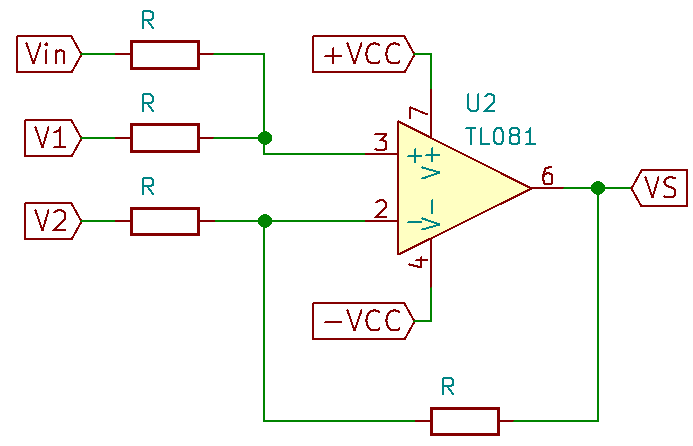
\includegraphics[width=8cm]{images/universel_sommateur.png}
\end{center}
}

%%%%%%%%%%%%%%%%%%%
\encadreTDExo{3 - Filtrer une composante fréquentielle autrement}{

\subsection*{Capacité commutée}

On se propose d'étudier la structure suivante, dont l'interrupteur $K$ est piloté par le signal de commande ci-dessous :

\begin{center}
	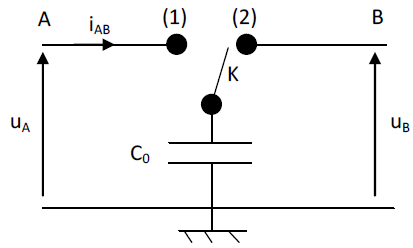
\includegraphics{images/capa_comm.png} 
	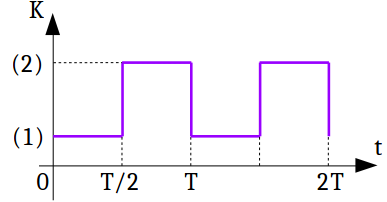
\includegraphics{images/capa_comm_signal.png}
\end{center}

\medskip

\begin{enumerate}
	\item Calculer la charge stockée dans $C_0$ entre les instants 0 et $T/2$, puis entre les instants $T/2$ et $T$.
	\item Quelle quantité de charges passe de A vers B entre les instants 0 et T ?
	\item Calculer alors le courant moyen circulant du point A au point B pendant une période T. 
	\item Donner l'expression de la résistance équivalente $R_{AB}$ vue entre les bornes A et B de cette cellule.
\end{enumerate}

\subsection*{Intégrateur}

On réalise un intégrateur à partir du circuit de la figure 2.

\begin{enumerate}
	\item Donner la fonction de transfert du circuit $T(j\omega) = u_2/u_1$ en fonction de $R_{AB}$ et de $C$.

\begin{center}
	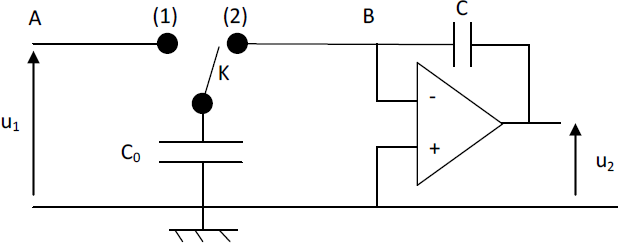
\includegraphics{images/capa_comm_integrateur.png}
\end{center}

	\item Que devient alors la fonction de transfert $T(j\omega{}) = u_2/u_1$ en fonction des éléments du système ($C_0$ et $C$) ?
	\item Quel est l'intérêt d'un tel circuit ?
\end{enumerate}

\subsection*{Etude du MAX296}

On s'intéresse au composant MAX296 dont une partie de la documentation technique est donnée en annexe.

\begin{enumerate}
	\item Quelles sont les fréquences maximales utilisables sur l'entrée \textsc{INPUT} ? Sur l'entrée \textsc{CLOCK} ? Quelles sont les applications visées ?
	\item Quelle fréquence faut-il appliquer sur l'entrée \textsc{CLOCK} pour avoir une fréquence de coupure de 3~kHz ? Que vaut alors l'amplification théorique du signal à : (a) 300~Hz ? (b) 30~kHz ? (c) 5~kHz ?
	\item Avec un filtre du second ordre (type Rauch) avec une pulsation de coupure à la même valeur, quelle aurait été l'amplification : (a) à 30~kHz ? (b) à 5~kHz ?	
	
\end{enumerate}

}


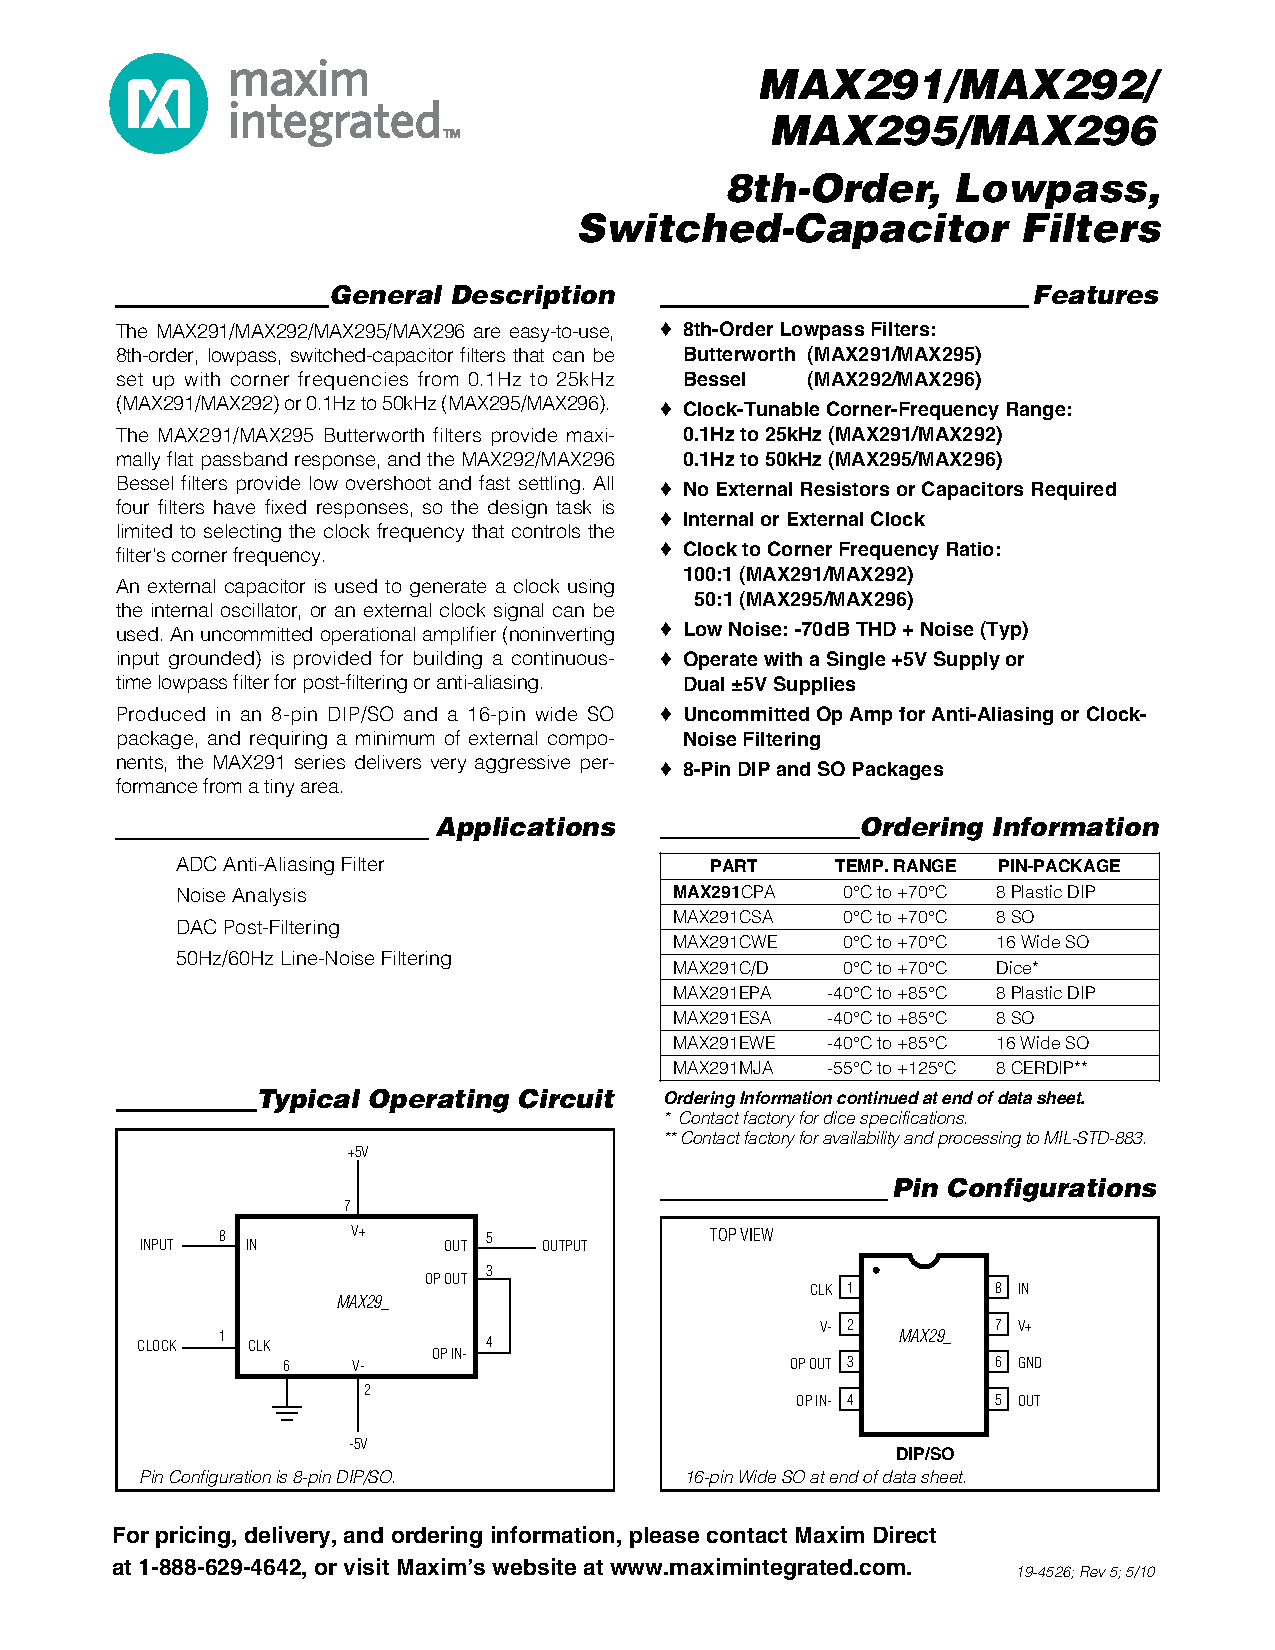
\includepdf[pages=-]{doc/MAX296.pdf}

\end {document}